\documentclass{exam}
\usepackage[exos]{main}

\title{Variations et extremums}
\date{29 Mars 2024}
\author{Seconde 9}

\pagestyle{empty}

\begin{document}
\maketitle
\thispagestyle{empty}
\begin{questions}
\question Soit $f$ une fonction à valeurs réelles. Pour chaque courbe représentative $\mathcal{C}_f$ de $f$ :
\begin{parts}
\part Donner l'intervalle de définition de $f$.
\part Dresser le tableau de variations de $f$.
\part Déterminer le maximum et le minimum de $f$, ainsi que les valeurs sur lesquels $f$ atteint ces extremums.
\end{parts}
\vspace*{1cm}
\begin{minipage}{0.45\textwidth}
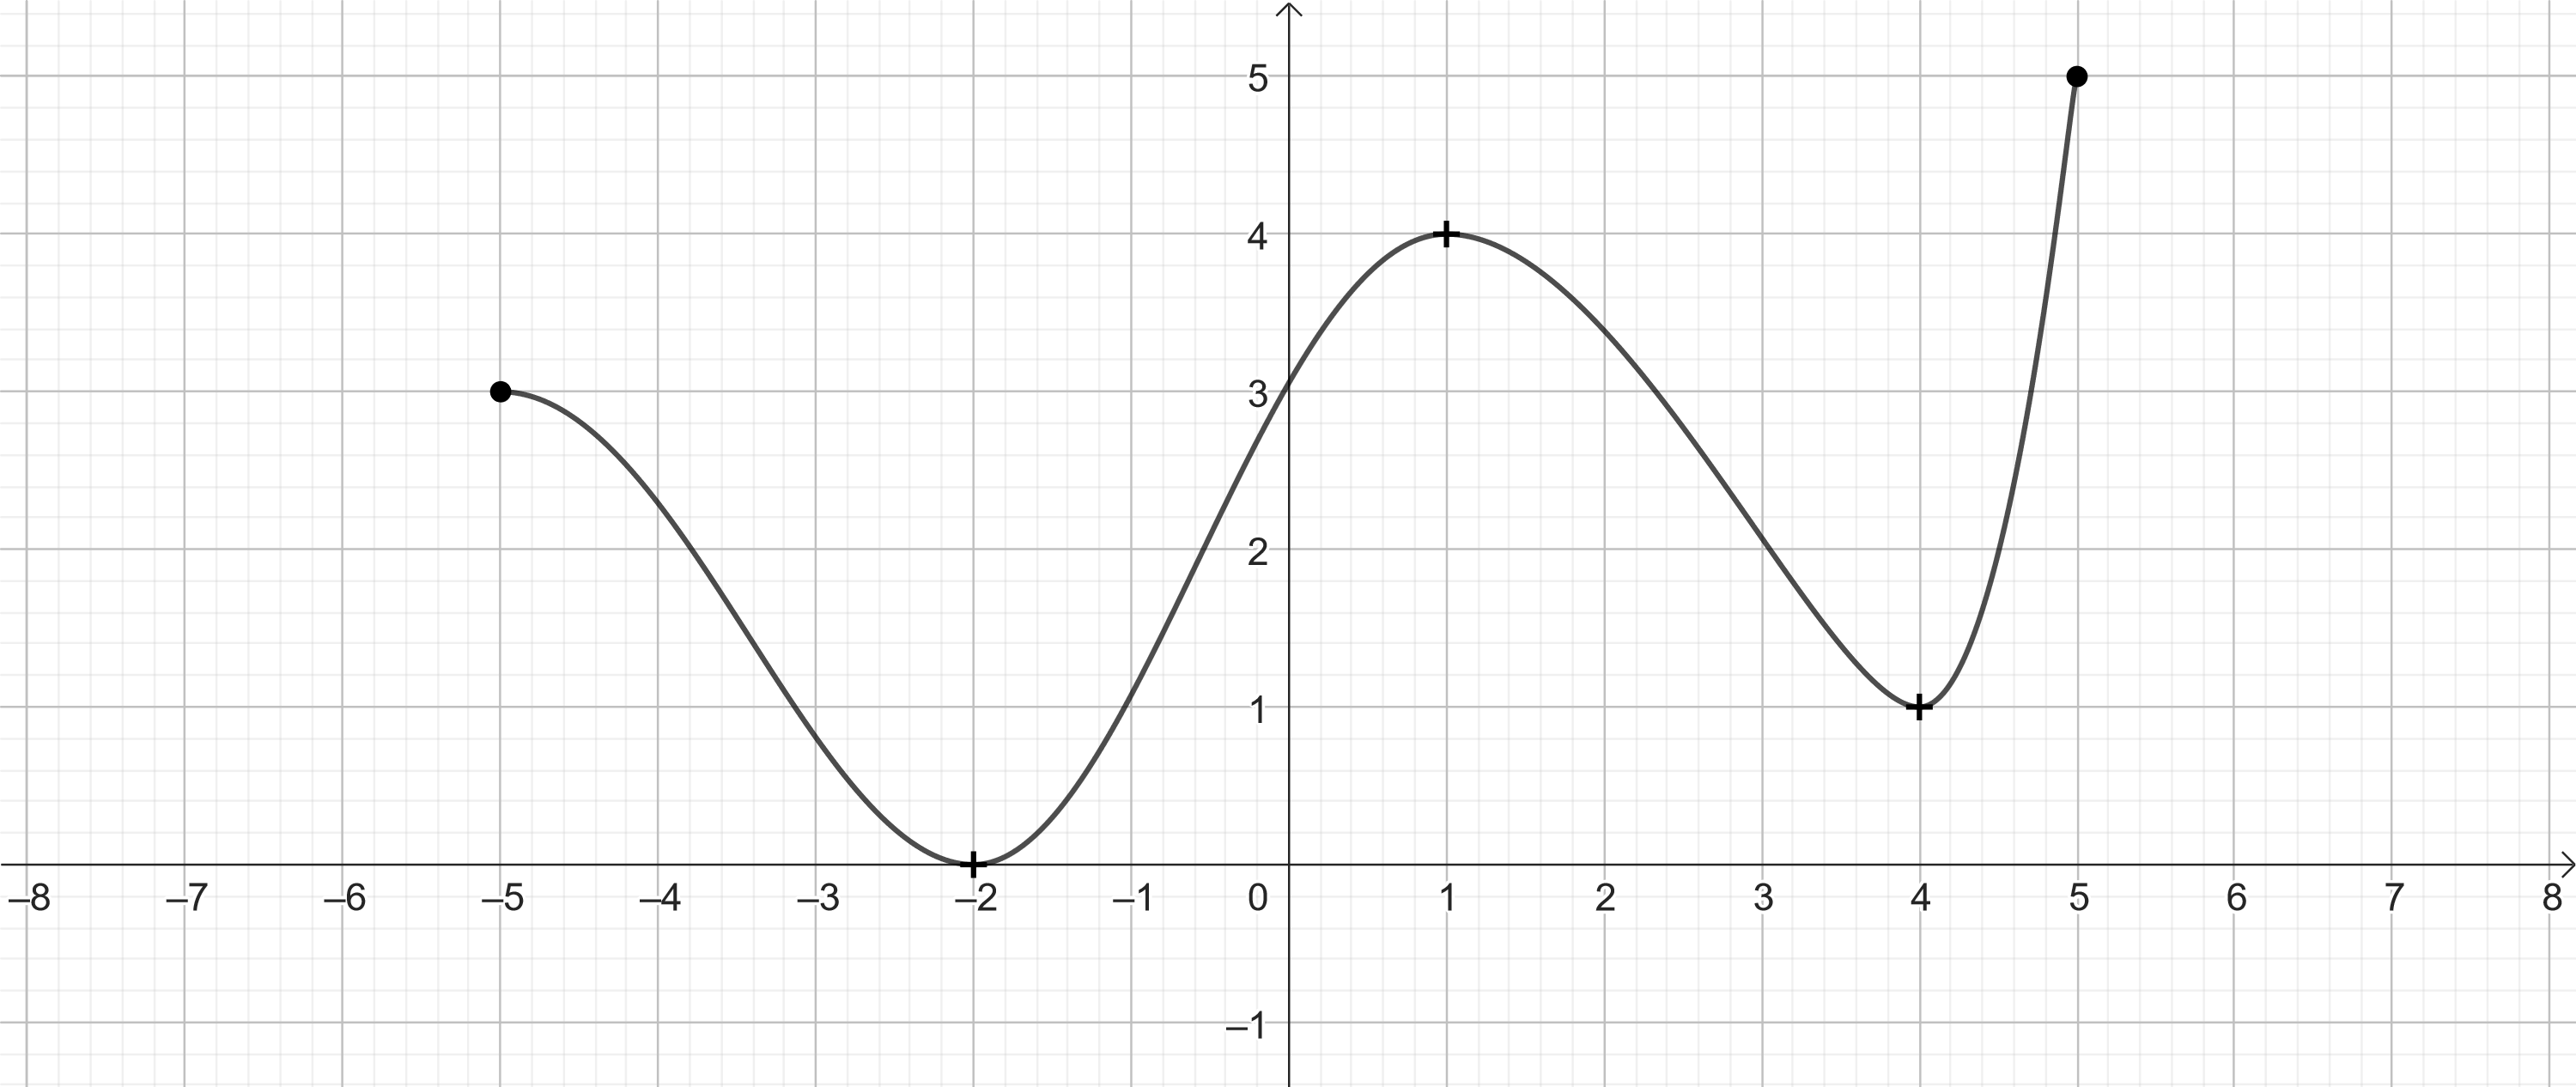
\includegraphics[width=\textwidth]{Fonction1.png}
\end{minipage}\hfill
\begin{minipage}{0.45\textwidth}
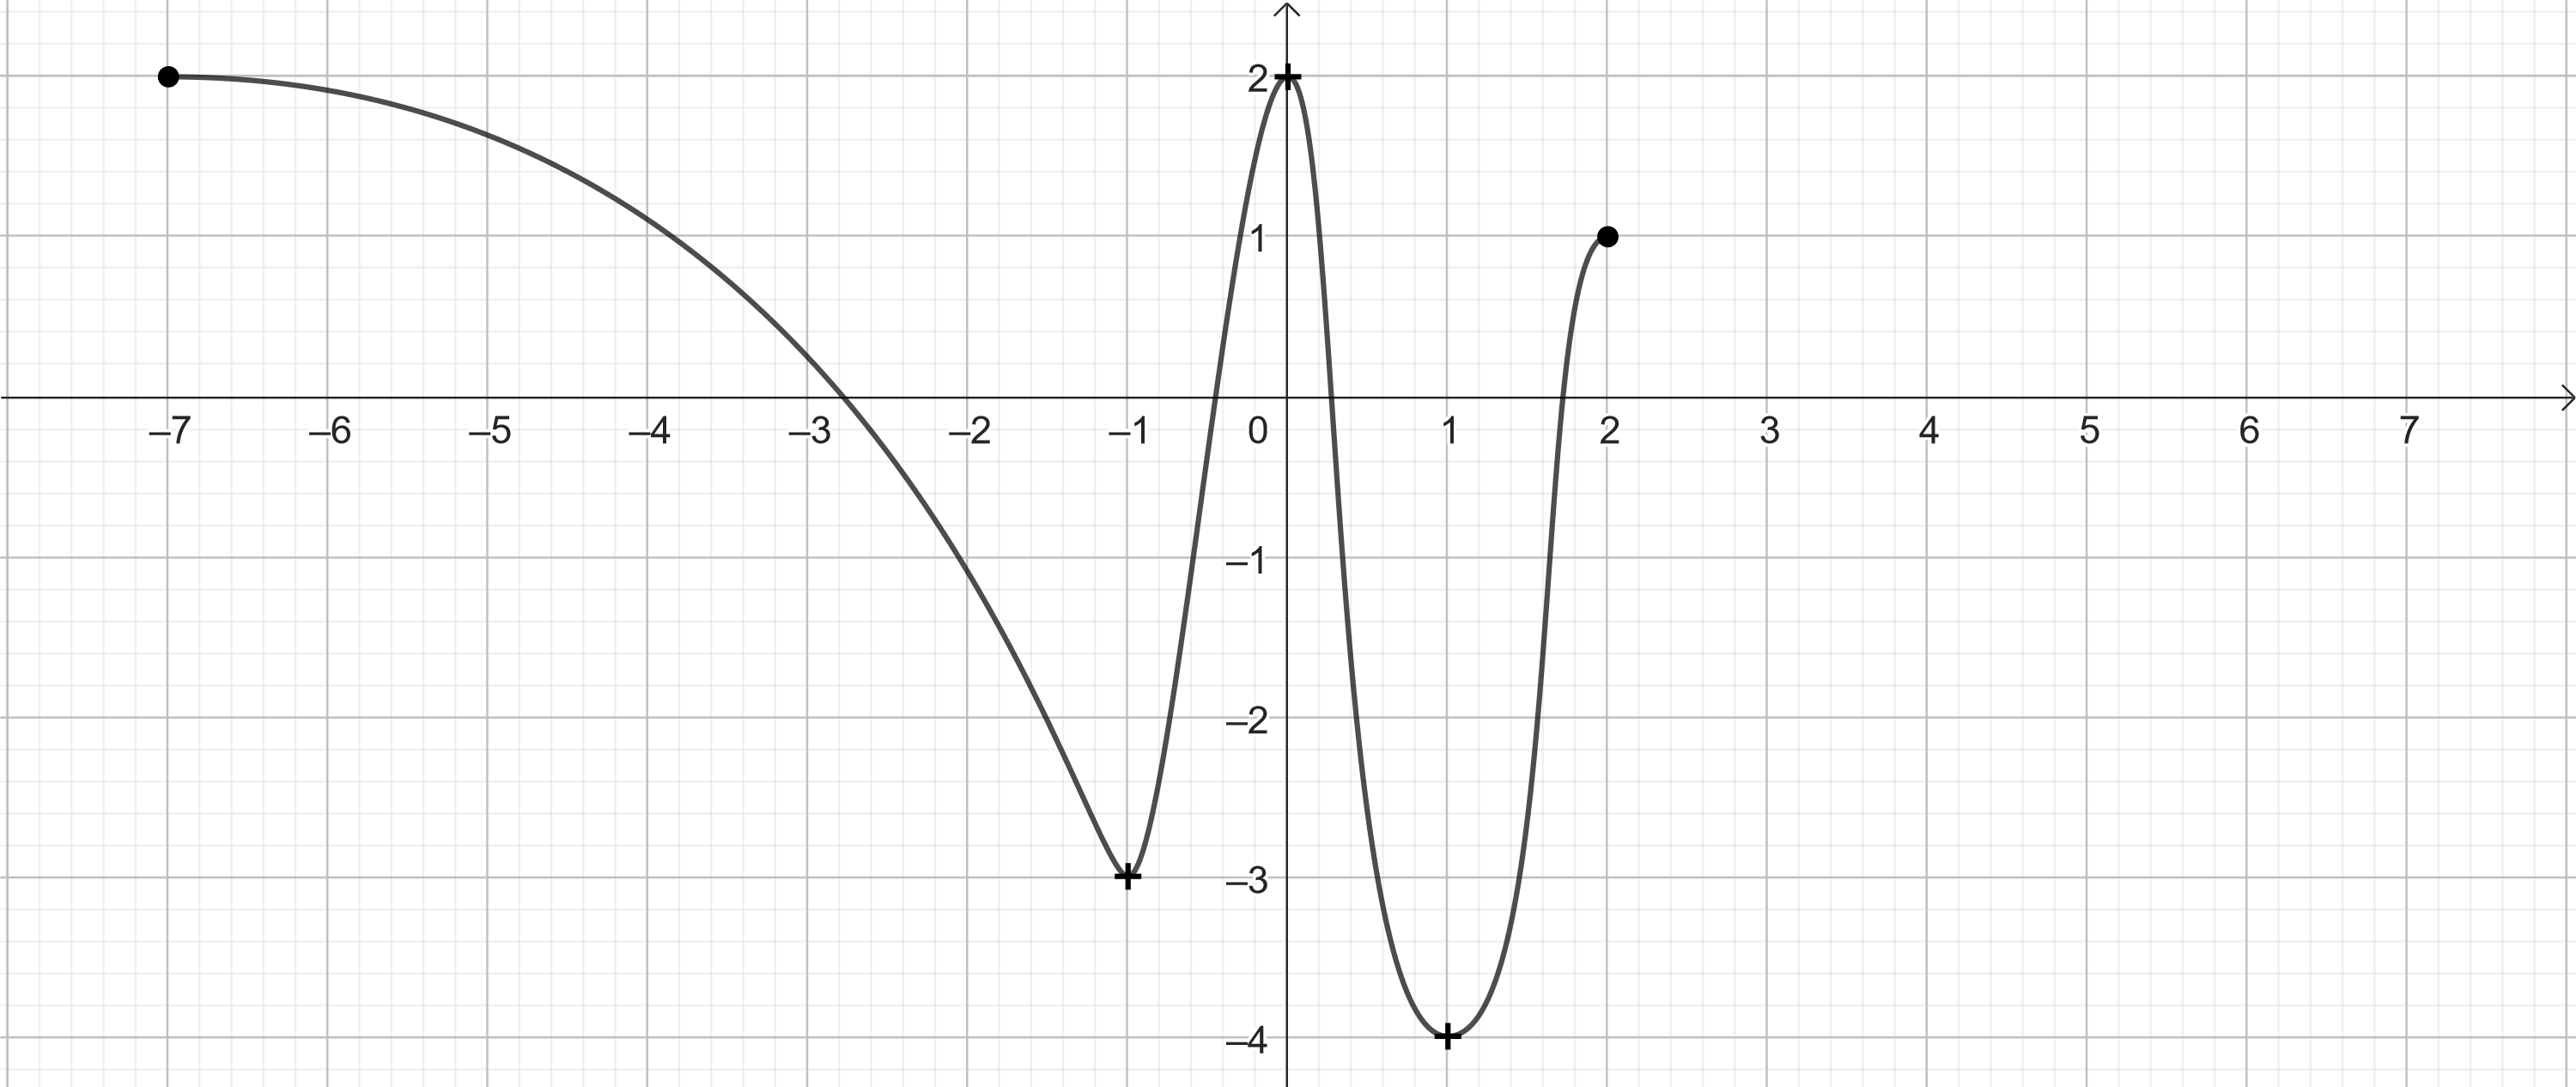
\includegraphics[width=\textwidth]{Fonction2.png}
\end{minipage}\hfill
\vspace*{1cm}
\begin{minipage}{0.45\textwidth}
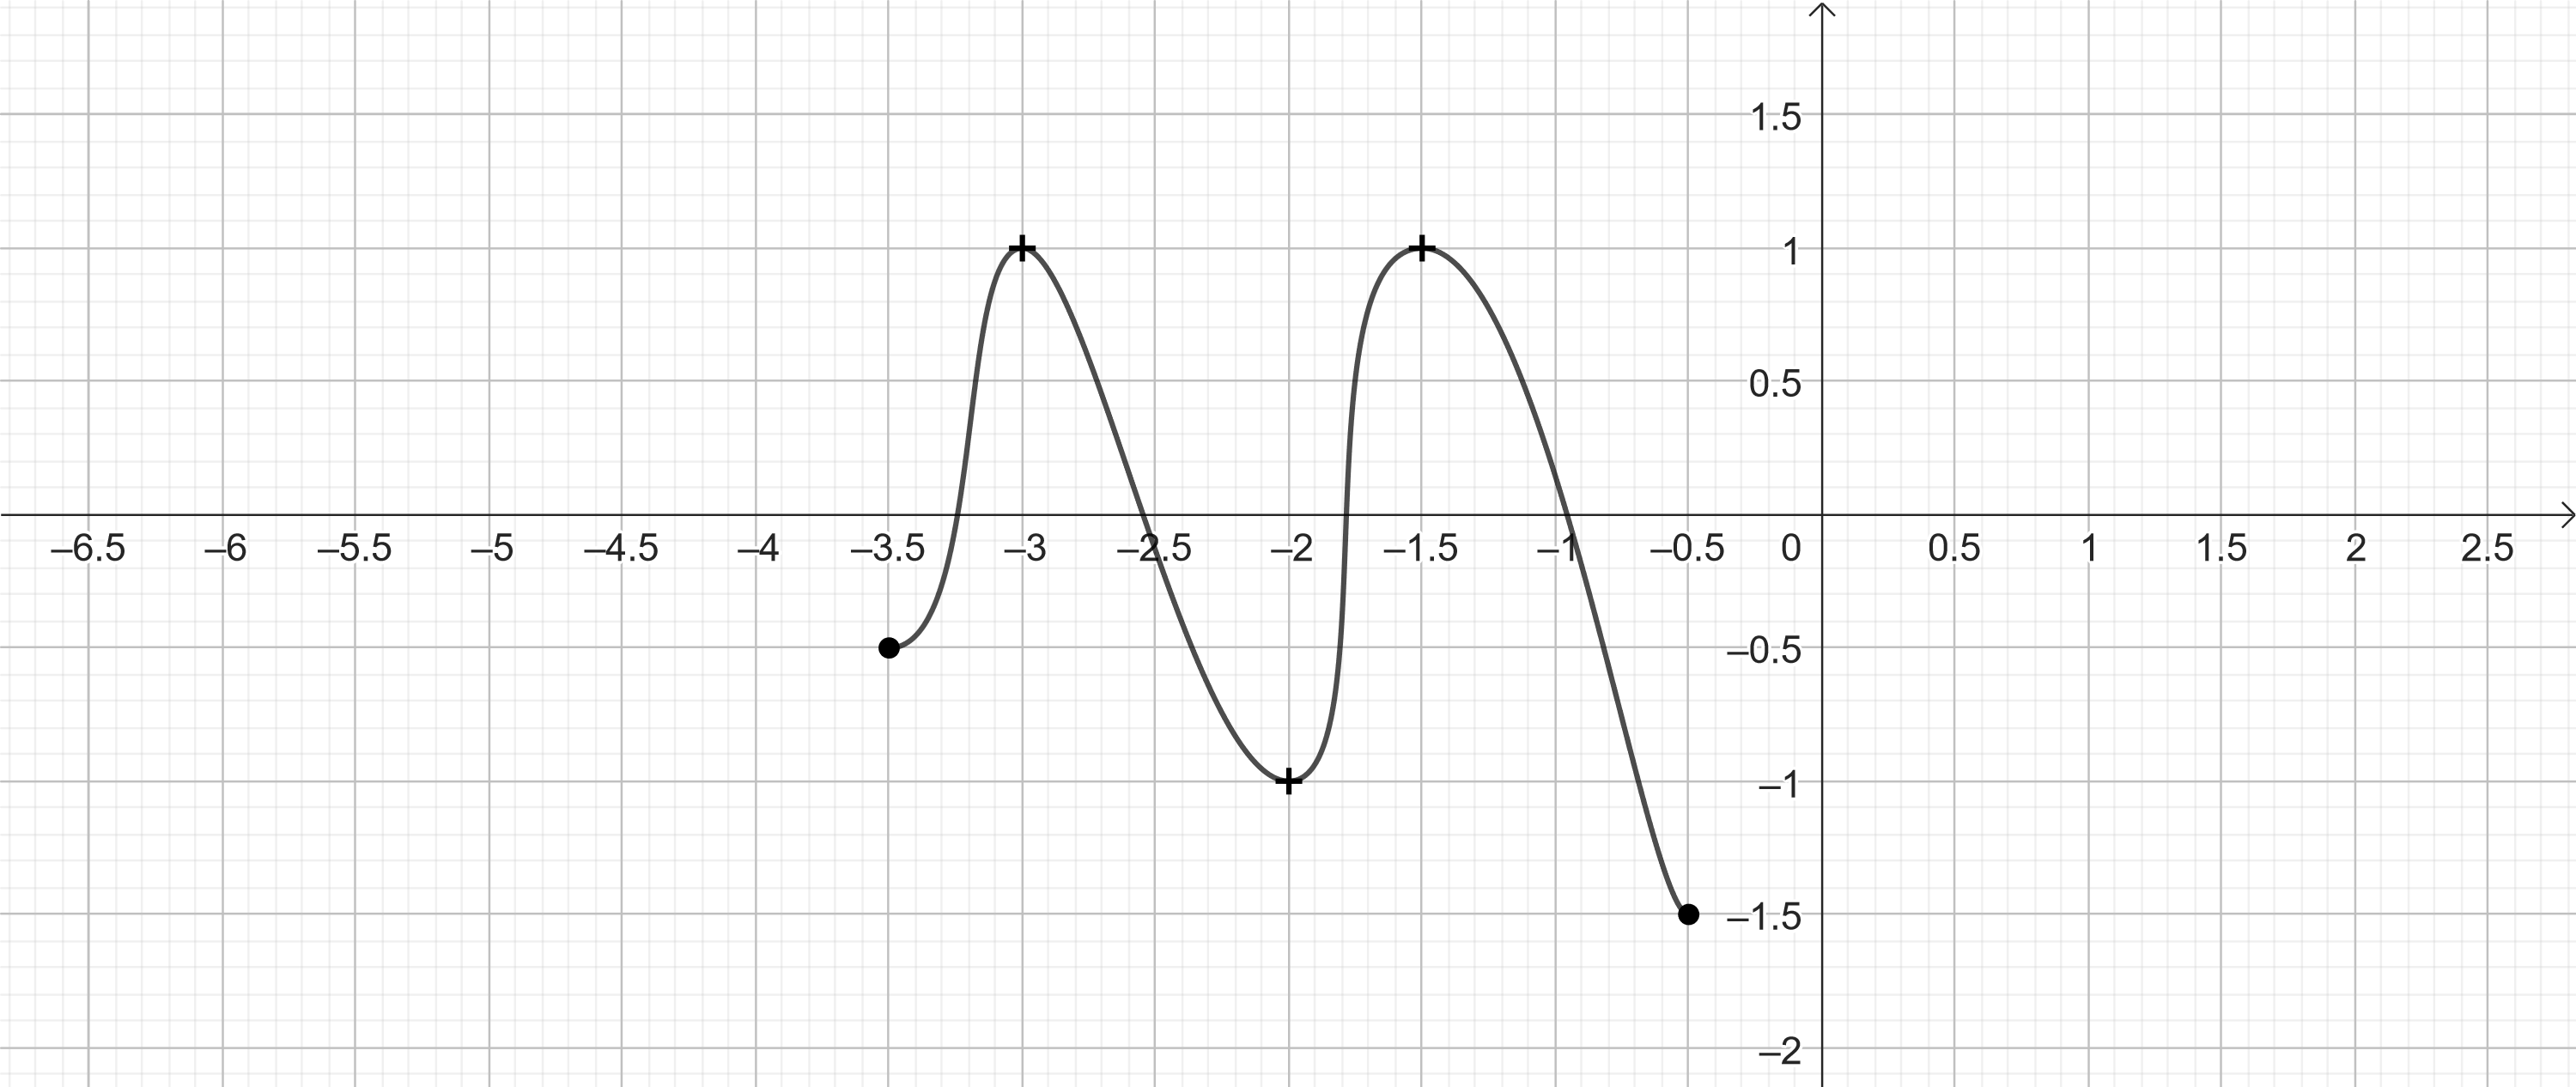
\includegraphics[width=\textwidth]{Fonction3.png}
\end{minipage}\hfill
\begin{minipage}{0.45\textwidth}
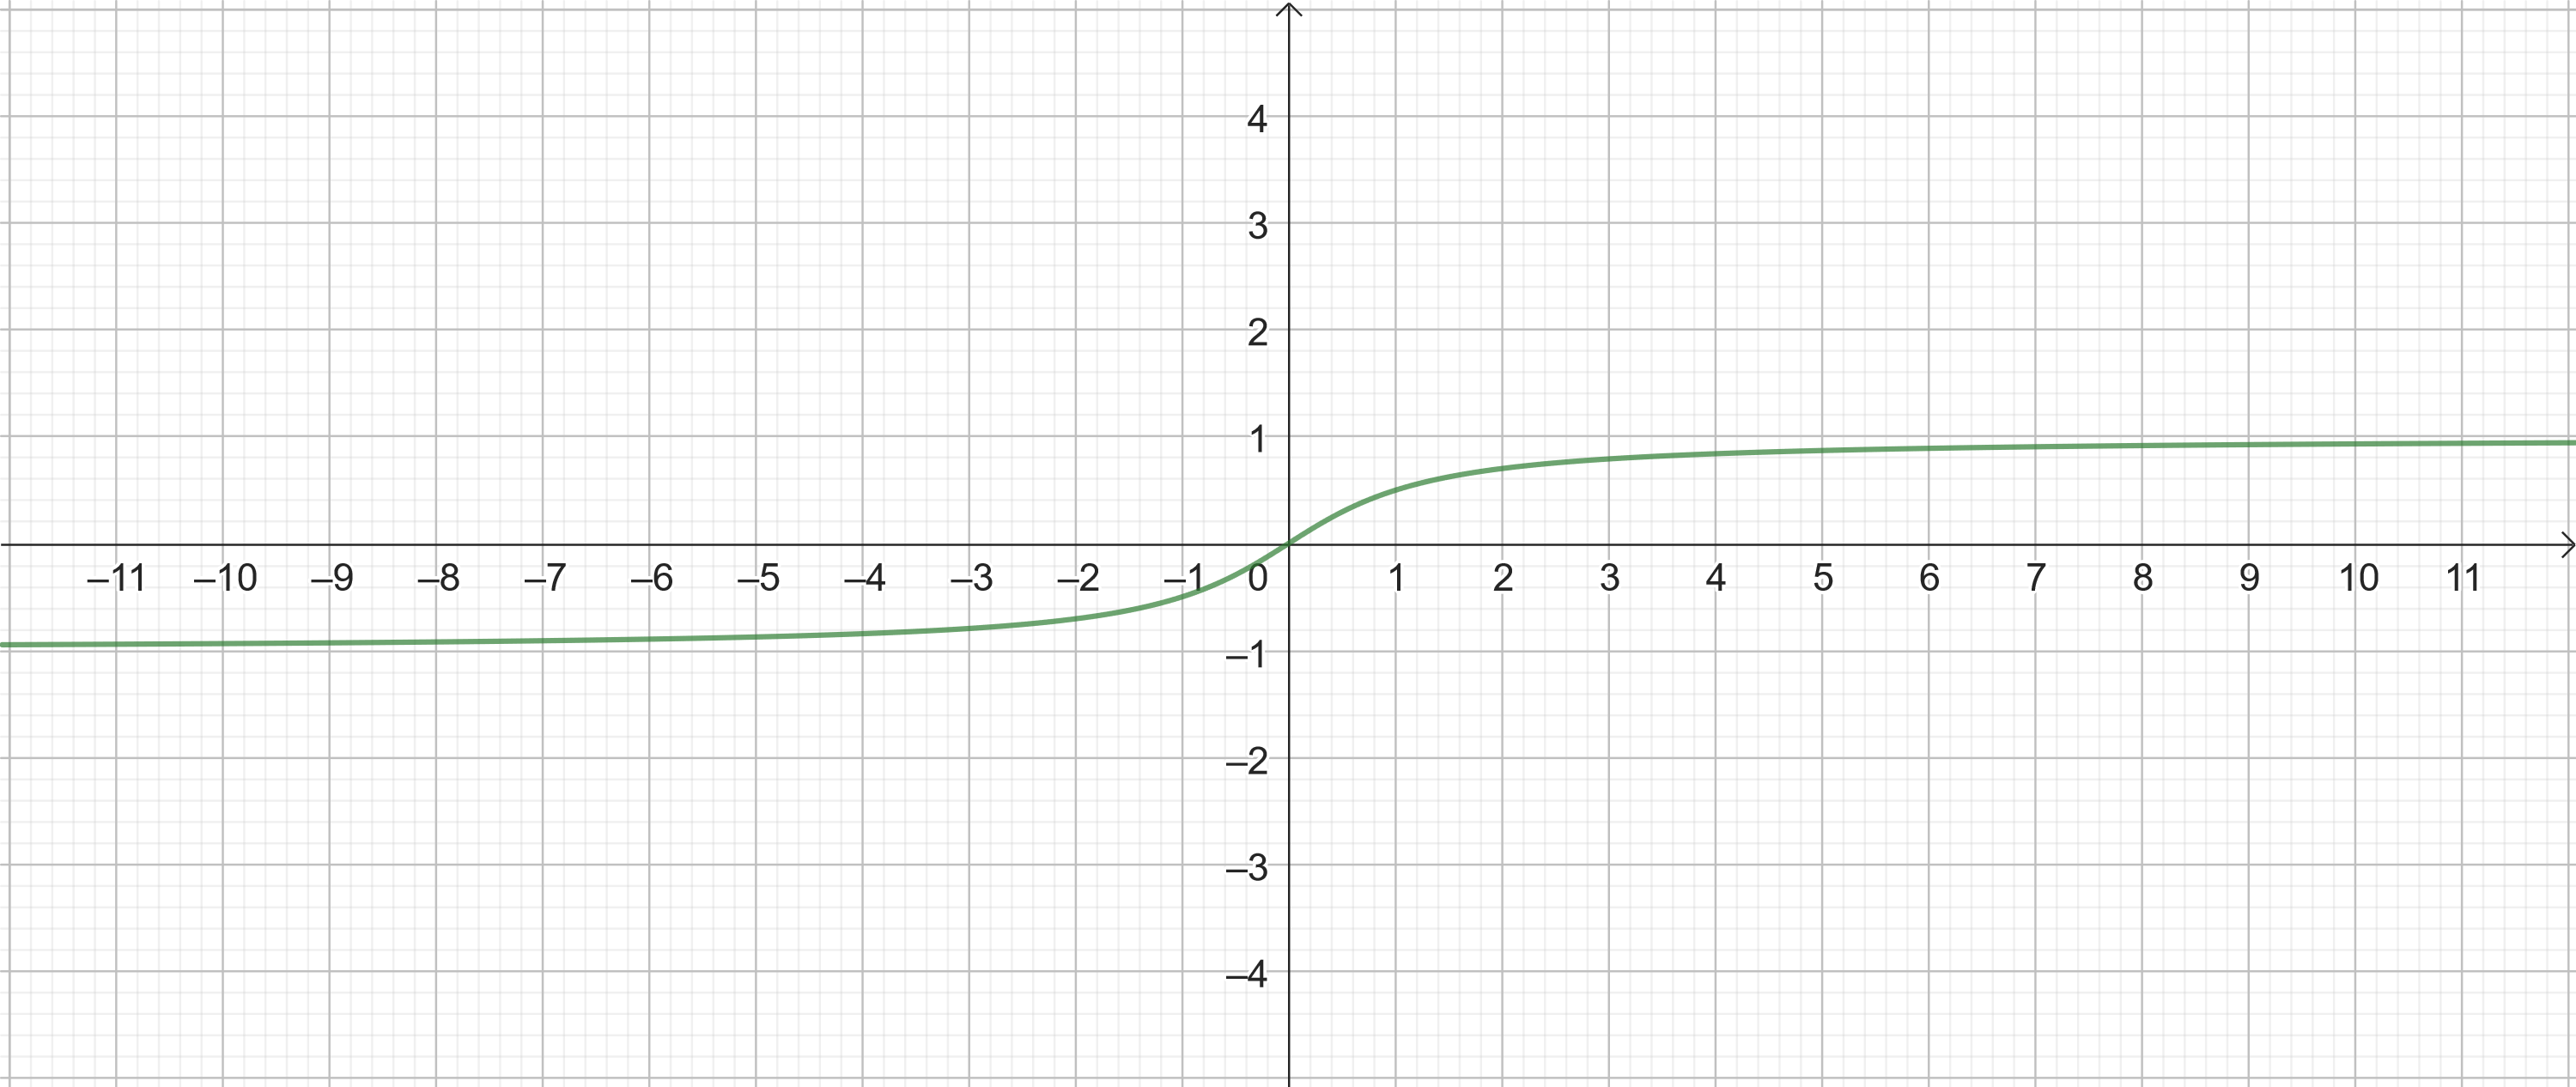
\includegraphics[width=\textwidth]{Fonction4.png}
\end{minipage}
\newpage
\question Soit $f$ une fonction à valeurs réelles. Pour chacun des tableaux de variations de $f$ suivants, déterminer le minimum et le maximum de $f$, ainsi que les nombres sur lesquels $f$ atteint ces extremums.
\begin{center}
\begin{tikzpicture}
\tkzTabInit{$x$/0.5, Variations de $f$/2}{$-5$,$0$,$3$,$10$}
\tkzTabVar{-/$-5$, +/$8$, -/$-6$, +/$9$}
\end{tikzpicture}
\begin{tikzpicture}
\tkzTabInit{$x$/0.5, Variations de $f$/2}{$-2$,$-1$,$6$,$8$}
\tkzTabVar{-/$-6$, +/$2$, -/$-4$, +/$8$}
\end{tikzpicture}
\begin{tikzpicture}
\tkzTabInit{$x$/0.5, Variations de $f$/2}{$-9$,$-2$,$8$,$10$}
\tkzTabVar{+/$9$, -/$-3$, +/$4$, -/$-10$}
\end{tikzpicture}
\end{center}
\vspace*{1cm}
\question Soit $ABCD$ un rectangle tel que $AB = 10$ et $AB = 6$. Soient $M$, $N$, $P$, $Q$ quatre point respectivement sur les segments $[AB]$, $[BC]$, $[CD]$ et $[DA]$ et tels que
\begin{equation*}
AM = BN = CP = DQ\,.
\end{equation*}
On note $a \in \left[0;6\right]$ la longueur $AM$.
\begin{center}
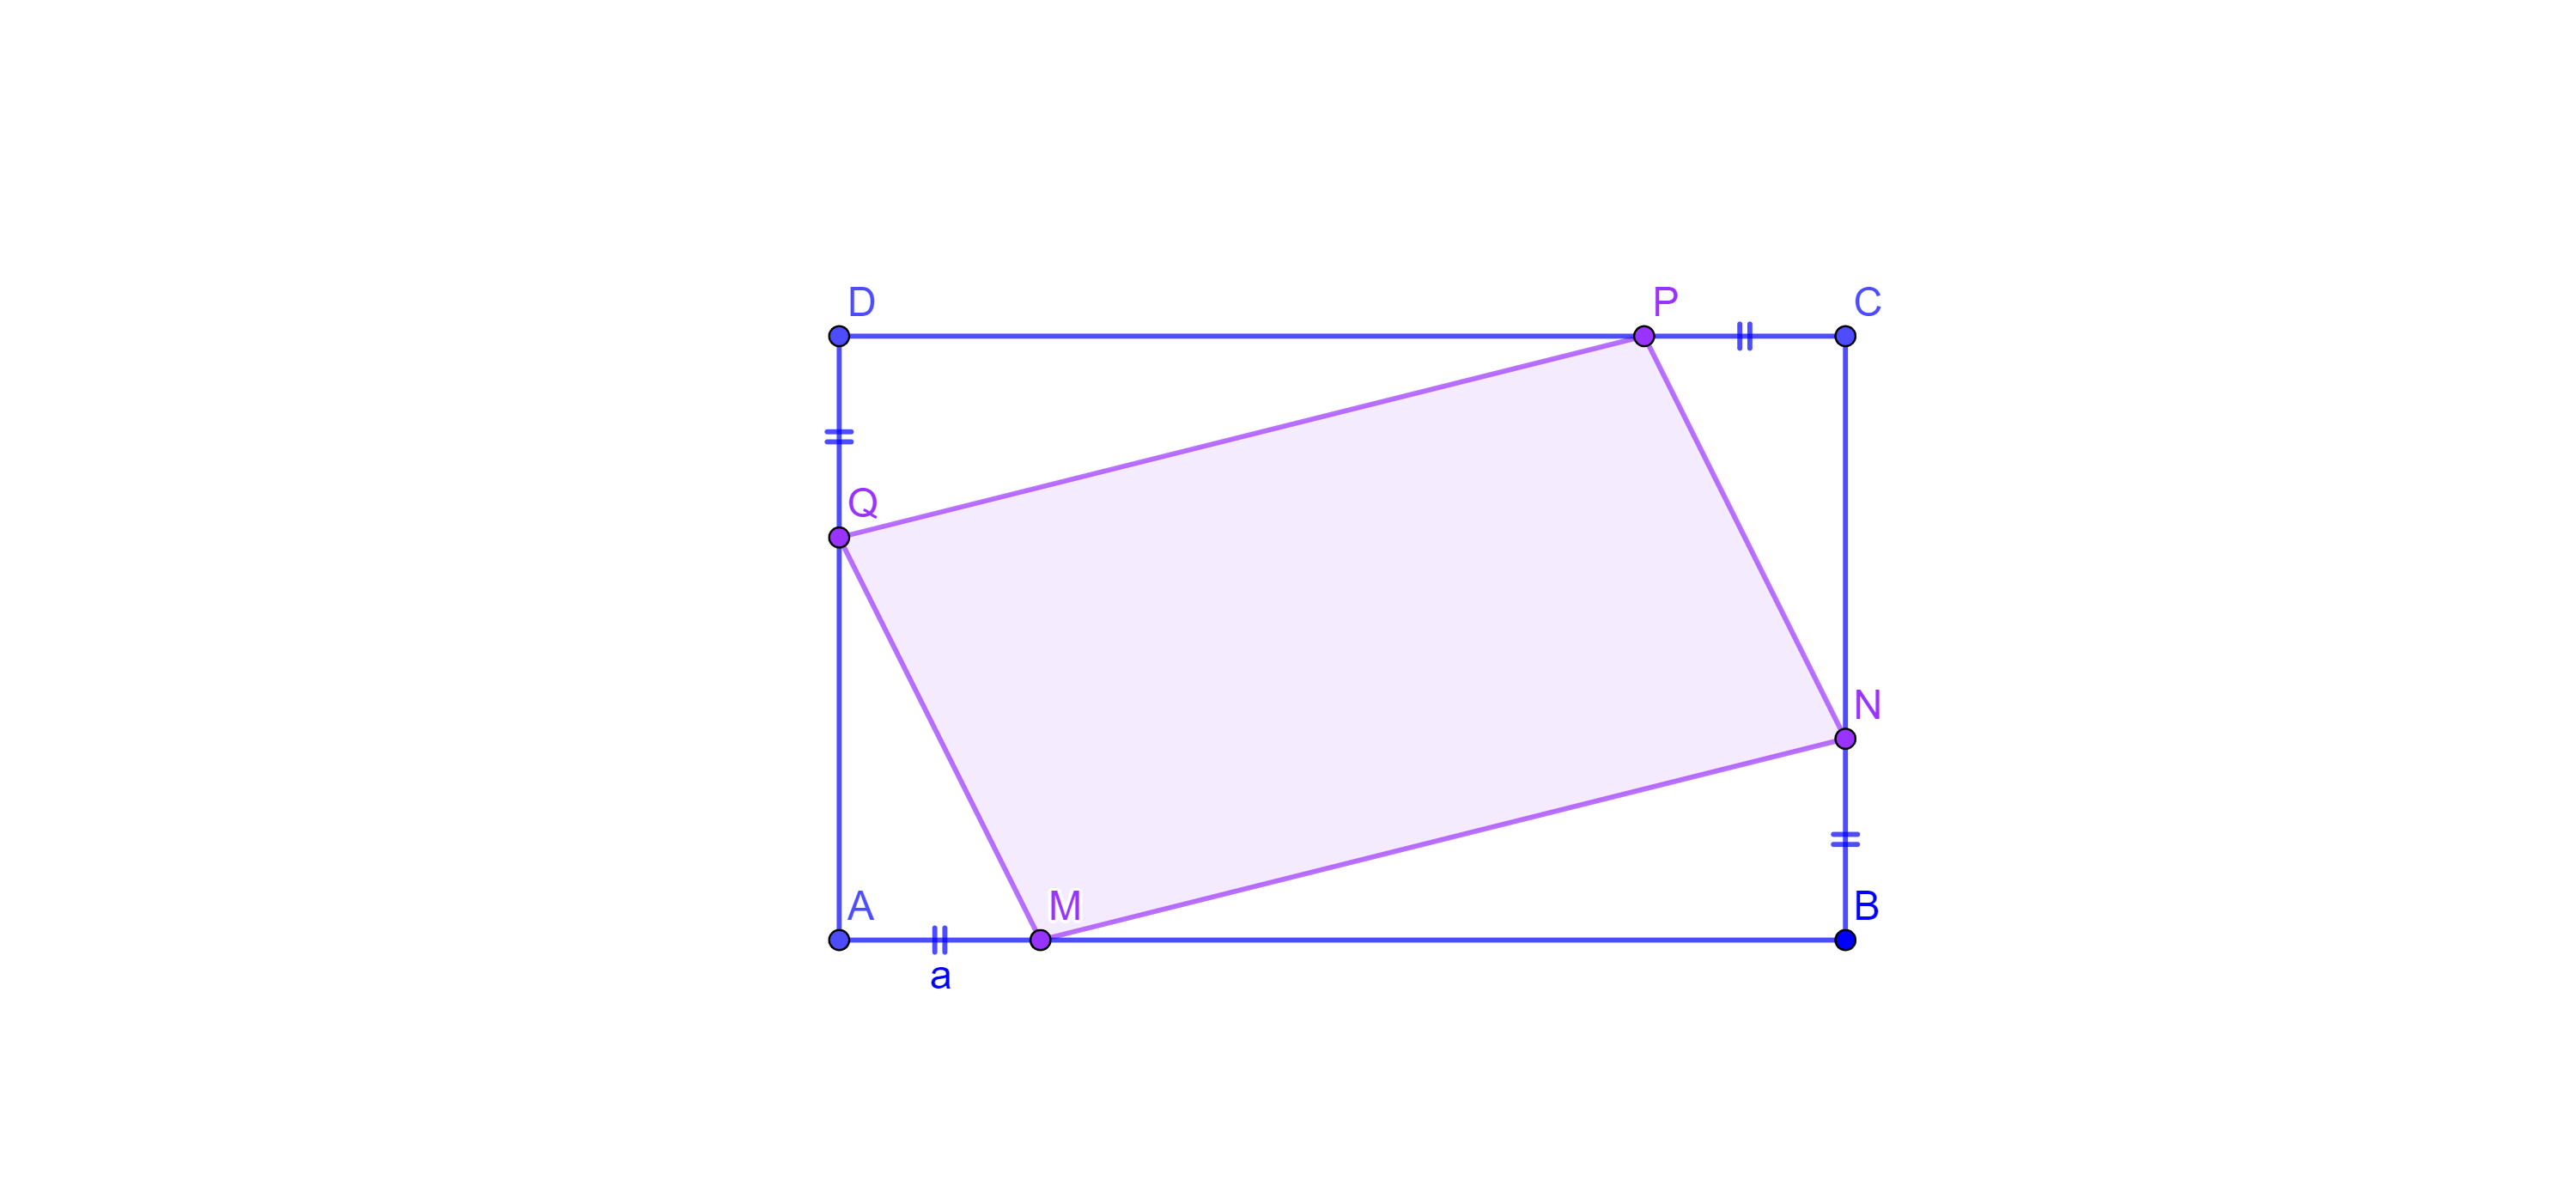
\includegraphics[scale=0.6]{Exercice3.png} 
\end{center}
\begin{parts}
\part Montrer que l'aire de $MNPQ$ en fonction de $a$ vaut
\begin{equation*}
2a^2 -16a + 60\,.
\end{equation*}
\part Montrer que cette aire vaut aussi
\begin{equation*}
2(a - 4)^2 + 28\,.
\end{equation*}
\part Justifier que cette aire est toujours supérieure à $28$.
\part En déduire l'aire minimale de $MNPQ$ en fonction de $a$, et pour quelle valeur de $a$ ce minimum est atteint.
\end{parts}

\end{questions}
\end{document}